\section{Composition and Phase Stability}
\label{sec:composition}

Composition determines which lithium sites are occupied, which framework sites are substituted and how much lithium is available during firing. Early LLZO studies established that Al, Ga, Ta, Nb, Y and related substitutions can stabilize a cubic-like garnet state or alter the tetragonal--cubic transition, but the concentration that maximizes conductivity is route-dependent \cite{puente2021garnet,raju2021crystal,anderson2024comprehensive,aote2023enhancement,siddiqui2024increased}. A composition label is therefore a starting hypothesis, not a guarantee of phase or carrier concentration.

\subsection{Dopant roles and lithium occupancy}

The most reproducible composition-level observation is that aliovalent dopants change both framework charge balance and the number of mobile lithium ions. Broad screening finds that dopants occupying different crystallographic sublattices produce distinct combinations of phase stability and transport, while co-doping can improve conductivity but also broaden the range of secondary phases \cite{anderson2024comprehensive,aote2024effect,aote2024investigation,aote2023enhancement,xu2023co}. Nb- and Ta-containing systems are especially sensitive to lithium inventory and thermal history, so nominal stoichiometry should be paired with post-processing elemental analysis \cite{luo2025phase,siddiqui2024increased,moy2025irreversible}.

Al-stabilized LLZO illustrates the coupled problem. High-temperature diffraction tracks phase evolution in Li$_{6.25}$Al$_{0.25}$La$_3$Zr$_2$O$_{12}$, and processing studies show that lithium volatilization changes the phase sequence as sample thickness and exposure geometry change \cite{gullbrekken2025phase,montoya2024lithium,heywood2023tailoring}. The practical implication is to report the lithium excess relative to the weighed batch, the covered area, the pellet thickness and the measured retained composition. A high conductivity measured after uncontrolled lithium loss cannot be assigned solely to the dopant.

Primary composition studies extend this picture across the dopant space. Ce substitution in Ga-doped LLZO, NbO$_2$-derived Nb substitution and Nb-doping studies each report coupled changes in lattice parameters, local electronic structure and electrochemical response \cite{aote2025impact,saran2026nbo2,yadzo2025improving}. Cluster-expansion calculations for Ta-doped tetragonal LLZO and phase-formation studies of LLZNO/LLZTO provide composition-specific hypotheses, but they still require diffraction and retained-element measurements on fired pellets \cite{maphoto2023phase,li2025phase,song2026effect}. Machine-learning molecular dynamics can rank local transport environments, yet its predictions are not substitutes for a measured phase fraction or conductivity \cite{kulkarni2025machine,xu2026rational}.

\subsection{Local phase relations and the missing global diagram}

A combined experimental--computational study maps a local Li$_2$O--La$_2$O$_3$--ZrO$_2$ relation, while high-temperature work resolves composition-specific phase transitions \cite{hong2024combined,gullbrekken2025phase}. These results are valuable local constraints, but they do not constitute a complete LLZO phase diagram spanning dopant content, lithium activity, oxygen potential and temperature. The literature should consequently distinguish a measured phase sequence from a phase-field extrapolation. The most useful next measurement is a small, compositionally spaced set of high-temperature diffraction and calorimetry experiments with quantified lithium retention, anchored to the local relations already reported.

Earlier structure determinations establish the reference states against which these newer substitutions should be compared. Tetragonal LLZO, aluminum-free cubic LLZO and zirconium-site Ge, Te or Y substitutions show that lithium distribution and framework distortion can change without a one-to-one correspondence between symmetry and total conductivity \cite{awaka2009synthesis,xie2011lithium,hu2018structure,deviannapoorani2013lithium,murugan2011high}. Reports of Ga stabilization, simultaneous Y/Ta substitution and Al-free Ta phase stability similarly demonstrate that dopant valence and lithium inventory must be interpreted together \cite{wolfenstine2012synthesis,elshinawi2012stabilization,dhivya2014effect,thompson2014tetragonal}.

\begin{figure}[t]
  \centering
  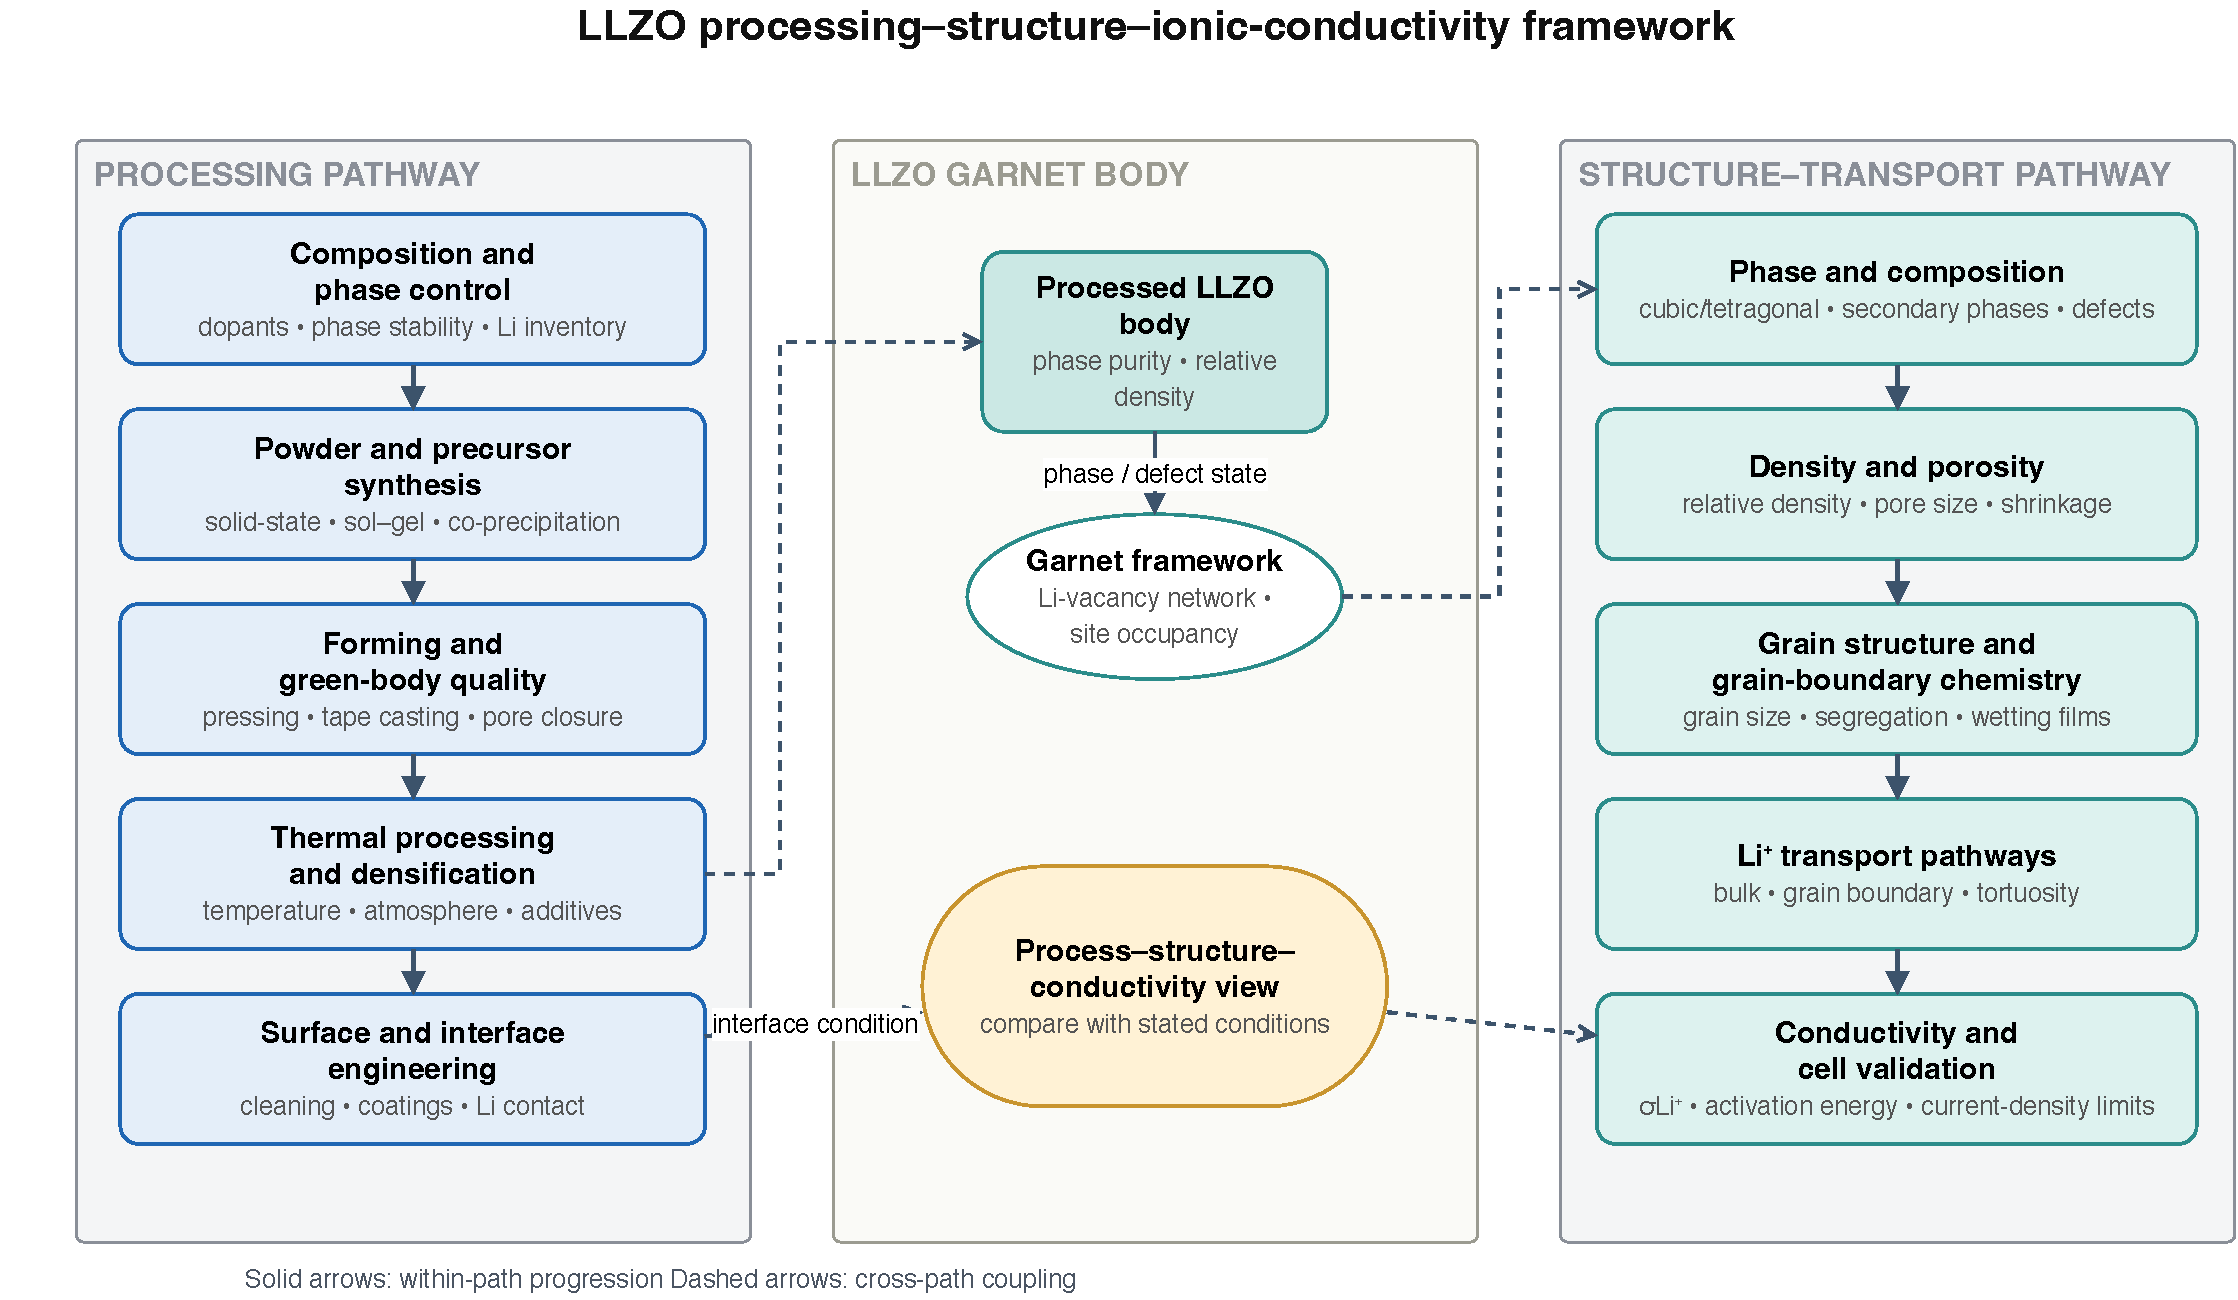
\includegraphics[width=0.96\linewidth]{../figures/pdf/fig1_processing_structure_conductivity.pdf}
  \caption{Process--structure--conductivity map used throughout this review. Precursor chemistry and lithium activity shape phase assemblage; forming and thermal history set density and interfaces; these states determine the resistance components measured in a cell.}
  \label{fig:process-map}
\end{figure}

\begin{table}[t]
\centering
\caption{Composition-level observations and the accompanying record needed for comparison.}
\label{tab:composition}
\begin{tabular}{P{0.20\linewidth}P{0.29\linewidth}P{0.25\linewidth}P{0.18\linewidth}}
\toprule
Composition lever & Recurrent observation & Required structural readout & Representative sources \\
\midrule
Al, Ga or multi-dopant substitution & Cubic-state stabilization is coupled to lithium occupancy and defect disorder & Phase fraction, dopant site/amount, retained Li & \cite{anderson2024comprehensive,aote2023enhancement,puente2021garnet} \\
Ta or Nb substitution & Conductivity and phase evolution depend on lithium inventory and thermal history & High-temperature diffraction, elemental retention & \cite{luo2025phase,siddiqui2024increased,moy2025irreversible} \\
Lithium excess or compensation & Excess can support phase formation but also increases volatilization and carbonate risk & Weighed excess, cover geometry, post-fire Li assay & \cite{gullbrekken2025phase,montoya2024lithium,heywood2023tailoring} \\
\bottomrule
\end{tabular}
\end{table}
